\documentclass[12pt]{article}
\usepackage[spanish]{babel}
\usepackage{graphicx}
\usepackage[usenames,dvipsnames]{xcolor}
\usepackage{color}

%codigos: \begin{abstract} \end{abstract} es resumen
%nueva pagina \newpage
%colores predefinidos : white, black, red, green, blue, cyan, magenta, yellow
%\textcolor{blue}{text}
%\color{blue!20!black!30!green}{Prueba} mezcla de colores, conviene manejar solo 2 colores, es mas manejable



\begin{document}
{\centering
{\Large{Escuela Superior Polit\'ecnica del Litoral\\Facultad de Ingenier\'ia en Electricidad y Computaci\'on\\}}
\vspace{0.6in}

\includegraphics[scale=0.5]{espol.png}\\
\vspace{0.8in}
{\LARGE \textbf{\color{blue}{Grid Computing\\ Computaci\'on Distribuida}}\\
\vspace{0.5in}
\large{Kevin Marlon Calder\'on Barrera}
}

%---%
\newpage
{\raggedright
Investigaci\'on referente al tema de {\textbf{Grid Computing}} o tambi\'en conocido como computaci\'on grid o distribuida.\\
La divisi\'on de los temas y subtemas han sido realizados combinando diversos conceptos de ``Computaci\'on grid" de wikipedia y de ``Computaci\'on Distribuida:Grid Computing" de Benjam\'in Dom\'inguez Hern\'andez
}
\vspace{-0.2in}
\tableofcontents

%---%
\newpage
\section{Computaci\'on Distribuida}
\begin{abstract}
Alguna vez alguien habr\'a imaginado lograr que los computadores puedan trabajar en equipo, m\'as de una vez se debi\'o encontrar problemas muy complejos para ser resueltos por un solo computador, de all\''i vemos la necesidad de compartir no solo datos o informaci\'on sino tambi\'en recursos, viendo tambi\'en el nacimiento de un nuevo concepto para la computaci\'on que es Grid Computing.\\
El nombre mismo nos indica a lo que esto se refiere, Grid Computing es una perspectiva diferente en el mundo de la computaci\'on, mirando a las computadoras no como varios equipos diferentes que pueden resolver problemas de poca complejidad pero separados, sino que ve a los computadores como verdaderos equipos que trabajan en unidad, logrando que las computadoras puedan trabajar en conjunto, como ser\'a observado mas adelante en el presente trabajo de investigaci\'on.\\
Para hacer una imagen sencilla de lo que es grid, lo podemos ver tambi\'en como una malla de algunos computadores que se unirán para qie se vean como un solo computador, con recursos de varios computadores a la vez.\\
Grid Computing es entonces parte importante de la computaci\'on distribuida que nos conviene bastante revisar y conocer acerca de estos conceptos para encontrar sus aplicaciones que sin duda alguna podr\'an ayudarnos a resolver problemas de mayor complejidad que los que pudieramos resolver sin utilizar la computaci\'on distribuida.\\
Todo nuevo conocimiento nos mostrar\'a mayor cantidad de soluciones a problemas actuales, nos armar\'a para enfrentar mejor problemas futuros y podremos ver que a\'un hay mucho mas por descubrir y conocer.\\
\end{abstract}

%---%
\newpage
\subsection{Objetivos de la investigaci\'on}
{\raggedright
\textbf{Objetivo General.-} \\\vspace{0.15in}Se busca dar a conocer conceptos claves acerca de Grid Computing, mostrar sus ventajas y sus aplicaciones.\\
\vspace{0.8in}
\textbf{Objetivos espec\'ificos.-} \\\vspace{0.15in}-Describir de forma clara y sencilla los conceptos de computaci\'on grid.\\
\vspace{0.2in}-Mostrar campos de aplicaci\'on de la computacion distribuida\\
\vspace{0.2in}-Diferenciar los distintos tipos de sistemas distribuidos y entender cual es la \\\hspace{-2.4in}aplicaci\'on espec\'ifica de cada uno de ellos.
}

%---%
\newpage
{\raggedright
\section{Conceptos B\'asicos de Grid Computing}
\subsection{Definici\'on}
Grid: Sistema paralelo y distribuido que permite la compartici\'on , detecci\'on y agregaci\'on de recursos ``aut\'onomos " geogr\'aficamente distribuidos. (Tomado de ``Computaci\'on Distribuida:Grid Computing" de Benjam\'in Dom\'inguez Hern\'andez) 
\vspace{0.2in}
\\Este paradigma fue propuesto a mediados de los noventa por Ian Foster y Carl Kesselman,no es un concepto nuevo pero tampoco es perfecto,hace falta protocolos y mejor estandarizaci\'on sin embargo la idea es bastante buena ,en sencillas palabras Grid es un sistema de computaci\'on que busca integrar en un conjunto los recursos de diversos computadores a la misma vez, a traves de ``middleware" que no es otra cosa que un software que brinda asistencia a la aplicaci\'on para que esta pueda comunicarse con otras aplicaciones, redes hasta hardware, ahorrando la tarea compleja de realizar la conexi\'on de un sistema distribuido. Esto nos permite realizar tareas complejas desde el ordenador utilizando recursos de otros.\\
Otra sencilla definici\'on que se puede dar a Grid Computing y como un concepto acertado es que este se refiere a la acci\'on de compartir tareas con otros equipos, utilizando cualquiera de sus recursos, sea procesamiento o simple almacenamiento de datos, sin importar el lugar geogr\'afico en el que se encuentren. Tambi\'en Grid suele ser traducido como ``Red".\\
Como se mencion\'o anteriormente la idea de Grid Computing fue concebida por Ian Foster y Carl Kesselman, quienes no solo dieron la idea, sino que dieron vida a la misma, ya que ellos mismos en conjunto desarrollaron las herramientas para que se puedan manejar las redes y trabajar en conjunto de una manera eficiente y flexible.

\subsection{Middleware}
El middleware es quien hace que sea posible la existencia del Grid y estas son sus principales funciones:
\begin{itemize}
\item[-]Encontrar el lugar conveniente para ejecutar la tarea solicitada.
\item[-]Optimizar el uso de recursos.
\item[-]Ejecutar las tareas.
\item[-]Monitorear el progreso de los trabajos en ejecuci\'on.
\item[-]Gestionar la recuperaci\'on frente a fallos.
\item[-]Dar aviso cuando se haya completado una tarea y entregar los resultados.
\end{itemize}
*Divisi\'on tomada de ``gridcomputing" de Ramon Millan.\\
\vspace{0.2in}
El Middleware como se puede observar, no tiene una tarea muy sencilla, por esta raz\'on no es tan solo un simple programa, sino que varios programas funcionan en conjunto como un solo software y se puede decir que ellos son los que ``arreglan o negocian" \hspace{0.01in} el uso de recursos de los proveedores.

\subsection{Organizaci\'on Virtual OV (VO por sus siglas en ingl\'es)}
La existencia de organizaciones virtuales, es de gran importancia en el enfoque de computacion grid.\\\vspace{0.1in}
``Una organizacion virtual es un conjunto de individuos y/o instituciones definida por reglas que controlan el modo en que comparten sus recursos."(Tomado de ``computaci\'on grid" de www.textoscientificos.com del apartado de redes)\\\vspace{0.1in}
Y un ejemplo de una de estas organizaciones es un porveedor de alg\'un servicio de aplicaci\'on que ayuda a analizar los datos cient\'ificos de un usuario en alg\'un lugar. Cabe tambi\'en recalcar que las organizaciones son diferentes las unas de las otras, porque cada una tiene un objetivo o simplemente busca resolver algo distinto.


\subsection{Actualidad}
Existen otros sistemas que buscan el compartir recursos, tales como el peer to peer(P2P, del cual se mencionar\'a luego), que teniendo en com\'un la idea de compartir recursos este tiene sus diferencias.
Tambi\'en existen programas a los cuales la computaci\'on grid ha brindado beneficios, las empresas que han notado la importancia que puede llegar a tener el ofrecer este sistema a sus clientes desarrollan software que permita hacerlo.
En la secci\'on anterior quedo definido lo que era un middleware, pero hay que resaltar que no existe tan solo un \'unico middleware, estos tienen diferentes funcionalidades, para realizar la conexi\'on dejando la posibilidad de escoger la m\'as adecuada para la situaci\'on.\\

\subsection{Ventajas y Desventajas}

\subsubsection{Ventajas}
Antes de mostrar las ventajas hay que indicar que es necesario que los usuarios esten enlazados entre si y los datos sean compartidos, asegurando tambi\'en que se puede ingresar a ellos en cualquier lugar y momento.\\
\begin{itemize}
\item[-]Se puede accesar a recursos desde nuestro computador.
\item[-]Muchos campos cient\'ificos resultan beneficiados por grid computing.
\item[-]El tiempo de an\'alisis en grandes cantidades de datos quedar\'a reducido, porque la capacidad de computo se eleva.
\item[-]Si por algun motivo los recursos o el ordenador que se esta usando se caen, la tarea que se estaba realizando se reasigan hacia otra maquina que cumpla los requerimientos para realizar esta tarea.
\item[-]Se aprovechan ciclos de procesamiento no utilizados de todos los ordenadores conectados en la red.
\item[-]Permite al usuario un acceso a recursos de datos y almacenamientos que puedan ser requeridos.
\item[-]Ayudar\'ia en la reducci\'on de costos, porque no ser\'ia necesario el gasto en provisionarse de supercomputadores cada cierto tiempo.
\item[-]Sin computaci\'on grid una organizacion solo podr\'ia usar recursos locales sobre los cuales tenga control.
\end{itemize}

\subsubsection{Desventajas}
Aun cuando la computaci\'on Grid es bastante buena presenta ciertos inconvenientes.
\begin{itemize}
\item[-]Necesita ser mas organizado en cuanto a pol\'iticas de seguridad.
\item[-]Las aplicaciones para el control del manejo de recursos debe desarrollarse m\'as.
\item[-]La computaci\'on grid deber\'ia poder manejar cualquier tipo de recurso.
\item[-]Necesidad de tener los servicios permanentemente conectados.
\item[-]Dificultad en sincronizar adem\'as de la adaptaci\'on de problemas a redes paralelas.
\end{itemize}
}

%---%
\newpage
{\raggedright
\subsection{Funcionamiento}
Un grid se define en una secuencia de pasos a realizar a traves de cada tarea, los cuales seran detallados en enumerados.
\begin{itemize}
\item[1.]El usuario tiene un problema un poco complejo para su sistema computacional individual, as\'i que necesita ayuda de otros sistemas. Implementa su tarea y se conecta al grid por medio de un software que ejecuta desde su equipo.
\item[2.]El ususario debe de acceder y ser validado, esto es por seguridad.\vspace{0.1in}\\\hspace{0.2in}
\textbf{Seguridad.-} La seguridad es muy importante, porque los recursos \\\hspace{0.3in}que son compartidos perenecen a persosnas distintas, entre los \\\hspace{0.3in}aspectos que se tienen en cuenta son las pol\'iticas que nos dir\'a que \\\hspace{0.3in}y a qui\'en se permitir\'a compartir, autenticaciones de ususarios y la \\\hspace{0.3in}autorizaci\'on.
\item[3.]Luego de su verificaci\'on de seguridad el usuario se podr\'a comunicar y conectarse a los recursos.
\item[4.]Se buscar\'a el servicio que sea mas adecuado para cada caso y una vez localizados se enviar\'a la tarea para que se ejecute a trav\'es del mismo.
\item[5.]El ususario podr\'a revisar el estado de su proceso, una vez terminado deben ser devueltos los resultados.
\end{itemize}
}

%---%
\newpage
{\raggedright
\section{Aplicaciones}
Segun ``Computaci\'on Distribuida:Grid Computing de Benjam\'in Dom\'inguez Hern\'andez" se tienen 5 campos de aplicaci\'on para la tecnolog\'ia grid.
\\
\subsection{La Supercomputaci\'on}
El sistema grid funciona con nodos en paralelo de modo que al unirse son como si fueran un solo nodo pero con mayor potencia par resolver problemas mas complejos y puntuales que no pueden ser resultos por un solo nodo apartado de la red.
Entre sus principales usos en este campo est\'an las simulaciones, el calculo y an\'alisis de grandes cantidades de datos.
\subsection{Sistemas Distribuidos en Tiempo Real}
Estos son sistemas que requieren de una respuesta inmediata y que la gran cantidad de datos generada pueda ser analizada al instante as\'i mismo como poder recibir actualizaciones del an\'alisis en tiempo real.
\subsection{Servicios Puntuales}
Son esos servicios que no queremos tener en nuestra organizaci\'on porque los vemos como de baja prioridad, pero a\'un asi es requerido que podamos acceder a ellos.
\subsection{Proceso Intensivo de datos}
Los datos viajan a trav\'es de la red y son distribuidos para que sean manejados por diferentes nodos, el uso principal de esto es que estos datos no pueden ser almacenados en un \'unico nodo.
\subsection{Entornos Virtuales de colaboraci\'on}
En base al uso de la potencia computacional que nos permite conseguir la malla del grid computing se crean los entornos virtuales 3D.\\
\vspace{0.2in}
Las instituciones y organismos que son mas atra\'idos para utilizar grid son aquellas que comparten un objetivo com\'un y encuentran mas efectivo para alcanzarlos el compartir y utilizar recursos compartidos.\\
Se ve repercusi\'on de los beneficios de usar grid en campos importantes para el desarrollo como lo son la medicina (para diagnosticos y an\'alisis), la ingenier\'ia que realiza simulaciones y an\'alisis de fallos, entre otras ramas m\'as que se ven beneficiadas.
Estas aplicaciones que se tiene de Grid Computing son aprovechadas actualmente por los cient\'ificos. Se espera que se pueda utilizar en el futuro en escala mundial, para que todos seamos usuarios a la vez que proveedores de los servicios o parte de estas organizaciones virtuales.\\
As\'i es como vemos que este sistema es utilizado por investigadores, cient\'ificos hasta m\'edicos, pero a\'un no ha llegado a manos de todos.\\
}

%---%
\newpage
{\raggedright
\section{Diferencia entre otros sistemas de computacion distribuida}
\subsection{Cloud Computing}
\subsubsection{Definici\'on de Cloud Computing}
A este concepto se le conoce como computaci\'on en la nube o servicios en la nube y este enfoque de sistema distribuido es acerca de los servicios, que estos e encuentren en internet y no los tenga que poseer el usuario.
La siguiente imagen tomada de wikipedia permitir\'a entender mejor lo que es cloud y a lo que se refiere que los servicios se encuentren en Internet o en una ``nube".\\
}
{\centering
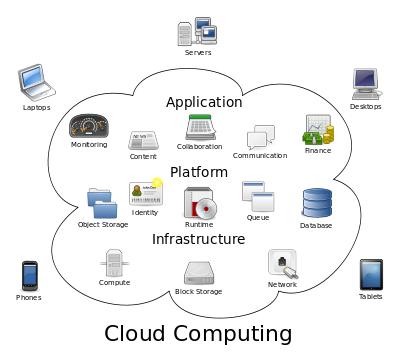
\includegraphics[scale=0.6]{cloud.png}
}\\
{\raggedright
\subsubsection{La Diferencia}
Grid Computing suele ser confundido con Cloud Computing, por esta raz\'on es necesario expanderse para tener mejor conocimiento y poder diferenciar el uno del otro, adem\'as de saber cual ser\'a nuestra mejor opci\'on frente a un requerimiento.\\
\begin{itemize}
\item[-]Cloud Computing tiene sus servicios en la red y son mas abiertos a los usuarios que Grid.
\item[-]La computaci\'on en Grid une los recursos de varios ordenadores en una sola red,  Cloud presta los servicios en internet pero con un comportamiento diferente a Grid, puesto que no busca el procesamiento de datos.
\item[-]El sistema Grid es mas estable porque si se cae la organizacion virtual que esta prestando el servicio, se busca otra organizaci\'on que puede entrar en su lugar, en cambio Cloud si se cae el servidor principal, se cae el servicio.
\item[-]B\'asicamente el uso y objetivos de Grid son diferentes a los de computing, si bien ambos buscan la distribucion de un servicio utilizando la red, ambos tienen diferente aplicaci\'on.
\item[-]Grid requiere de un software que haga posible el compartir recursos dentro de la red, mientras que Cloud solo utiliza un software como m\'ascara, para accesar al servicio que se usara en internet.
\end{itemize}
}

%---%
\newpage
{\raggedright
\subsection{Peer-to-Peer (P2P)}
\subsubsection{Definici\'on de Peer-to-Peer}
Una red peer-to-peer o red de pares,tambi\'en llamada red entre iguales o por sus siglas en ingl\'es P2P, es una red en la que todos son clientes y servidores a la vez, los nodos son interconectados y son tratados como iguales para cada nodo de la red.
La mayor utilidad que se aprovecha de este tipo de redes es el de compartir archivos de cualquier tipo y lo hacen aprovechando y optimizando el espcacio de banda de los dem\'as usuarios de la red, tambi\'en en el momento de transmitir los datos, los nodos y el enlace tendr\'an mayor eficiencia dependiendo de la capacidad de almacenamiento y de la cantidad de usuarios que tengan el mismo recurso ya que se comportar\'an tambien como servidores.\\
En general este tipo de redes es descentralizada, pero estas redes pueden ser clasificadas por su grado de centralizaci\'on. Donde lo ideal o una red \\peer-to-peer pura es una totalmente descentralizada.\\
}
\vspace{0.2in}
{\centering
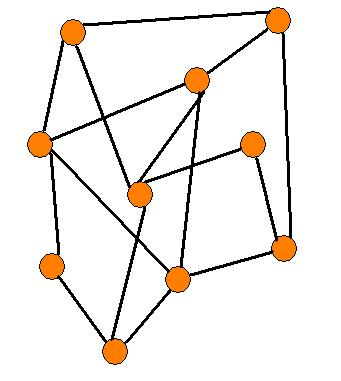
\includegraphics[scale=0.6]{P2P.jpg}\\
\small{Ilustraci\'on de como se ver\'ia una red peer-to-peer}
}\\

{\raggedright
\subsubsection{La Diferencia}
Grid Computing y peer-to-peer tienen similitudes, puesto que son bastantes descentralizadas y tienen el principio de formar una malla, pero tambi\'en existen diferencias que es necesario conocer para escoger el sistema adecuado cuando es necesario.\\
\begin{itemize}
\item[-]Grid Computing tiene un grupo de usuarios mas selecto que peer-to-peer, porque en Grid, se disponen a compartir por un objetivo similar, mientras que P2P comparte archivos a todos los de la red.
\item[-]El peer-to-peer se ha popularizado porque cualquiera puede pertenecer a esta red, se mantiene un nivel menor de seguridad dando posibilidad al anonimato y poca motivaci\'on al trabajo en conjunto.
\item[-]Los recursos de Grid son mas potentes y mejor conectados para trabajar de manera distribuida, con equipos de diversas clases, como una base de datos o equipos cient\'ificos, mientras que los recursos peer-to-peer son en su mayor\'ia t\'ipicos computadores.
\end{itemize}
}

%---%
\newpage
{\raggedright
\section{Conclusiones}
Esta investigaci\'on ha llevado al mejor comprendimiento de diversas definiciones y a llegar a un mayor conocimiento en cuanto a computaci\'on distribuida.\\
Fue necesario realizar la investigaci\'on completa y no solo del tema escogido porque muchos conceptos eran similares, por esta raz\'on necesitaba conocer mejor todo lo referente a computaci\'on distribuida para poder diferenciar a Grid Computing de los dem\'as sistemas de distribuci\'on.\\
A\'un as\'i toda esta investigaci\'on giro en torno a Grid Computing, solo que con una visi\'on m\'as amplia del mismo, viendo no solo lo que es Grid Computing sino tambi\'en lo que rodea al tema.\\
Se lleg\'o a la conclusi\'on que gracias al sistema grid es posible conseguir una supercomputadora, esto porque los recursos se comparten para realizar las tareas, todo como si se tratara de un solo computador.\\
Grid Computing necesita algunos requerimientos para ponerse en funcionamiento, como son las organizaciones virtuales y otro muy importante que es el middleware.\\
Middleware se trata de un software que hace posible la existencia de este sistema de redes en paralelo.\\
Finalmente Grid Computing es un sistema utilizado en el mundo cient\'ifico, por la misma dificultad que representa hacerlo, sin embargo no se pierde la expectativa que alg\'un d\'ia pueda ser m\'as conocido y se pueda utilizar por mayor cantidad de personas, todo est\'a en lograr concretar el conocimiento de seguridad del Grid y mostrar a los usuarios el potencial que represanta utilizarlo. De hecho ya hay empresas desarrolladoras de software que han puesto la mira en que llegue ese d\'ia
}

%---%
\newpage
{\raggedright
\section{Referencias}
\begin{itemize}
\item[-]Computacion Grid en wikipedia \\\hspace{0.1in}http://es.wikipedia.org/wiki/Computaci\%C3\%B3n\_grid
\item[-]Funcionamiento Grid Computing Basics  \ \hspace{0.1in}http://www.worldcommunitygrid.org/about\_us/viewGridComputingBasics.do
\item[-]Middleware en wikipedia \\\hspace{0.1in}http://es.wikipedia.org/wiki/Middleware
\item[-]Introducci\'on a computaci\'on en grid tomado de textos cient\'ificos.\\\hspace{0.1in}http://www.textoscientificos.com/redes/computacion-grid
\item[-]Grid Cpomputing por Ram\'on Mill\'an, funcionamiento y aplicaciones.\\\hspace{0.1in}http://www.ramonmillan.com/tutoriales/gridcomputing.php
\item[-]Computaci\'on Distribuida:Grid Computing de Benjam\'in Dom\'inguez\\\hspace{0.1in}http://biblioteca.usac.edu.gt/tesis/08/08\_0257\_CS.pdf
\\\vspace{0.2in}\textbf{Diferencias entre otros sistemas distribuidos.}
\item[-]Computaci\'on en la nube. Fuente: wikipedia\\\hspace{0.1in}http://es.wikipedia.org/wiki/Computaci\%C3\%B3n\_en\_la\_nube
\item[-]Cloud Computing vs Grid Computing desde brigthub\\\hspace{0.1in}http://www.brighthub.com/environment/green-computing/articles/68785.aspx
\item[-]Deferencia: Cloud Computing Grid Computing vs, publicado por Manuel. Fuente: hosting alojamiento\\\hspace{0.1in}http://hostingalojamiento.blogspot.com/2010/05/diferencia-cloud-computing-grid.html
\item[-]Peer-to-peer en wikipedia\\\hspace{0.1in}http://es.wikipedia.org/wiki/Peer-to-peer
\item[-]Diferencias entre el Grid y el P2P por Ram\'on Mill\'an\hspace{0.1in}
http://blogtelecomunicaciones.ramonmillan.com/2008/06/diferencias-entre-el-grid-y-el-p2p.html
\end{itemize}
}


%\begin{figure}[h]
%\centering
%\includegraphics[totalheight=2in,width=2.5in]{CVPicture}\\\vspace{0.1in}  %figuras extras para parte explicativa
%\includegraphics[totalheight=2in,width=2.5in]{Hao}
%\end{figure}

\end{document}